\chapter{Introduction}
\label{chap:introduction}

\section{Motivation}
Blimps are often used as advertising vehicle. Especially eye-catching are special shaped blimps, e.g. blimps that have the shape of a mascot, car or any other commercial product (see figure \ref{fig:blimps}).
An alternative are conventionally shaped blimps showing imprints or banners.
The arrangement of the actuators for those different shaped blimps varies a lot and needs in general manual adjustment of the control algorithm.
Using some adequate sensors, it would be useful to determine the effect of an actuator on the movement of the blimp automatically.
With such an algorithm, the blimp hull can be manufactured independently on the actuation which just can be attached to the blimp and the controller figures out the effect of its actuators by its own.
This procedure is illustrated in figure \ref{fig:motivation}.

\begin{figure}[hbtp]
\label{fig:blimps}
\centering
\includegraphics[width=.4\linewidth]{images/CustomBull_Lg.jpg}
\includegraphics[width=.4\linewidth]{images/CustomCar.jpg}
\caption{Special shaped blimps are used for advertising \citep{rcblimps}.}
\end{figure}

\begin{figure}[hbtp]
\label{fig:motivation}
\centering
\includegraphics[width=.85\linewidth]{images/motivation.png}
\caption{The goal is to find an algorithm, that allow to take any blimp shape (\textit{left}) and put the actuation units (\textit{center}) on. The actuation configuration is then automatically detected, such that elegant movements can be performed without manual controller adjustments (\textit{right}).}
\end{figure}


\section{Configuration Estimation}
This work is on estimation of the actuation configuration for a multi-actuated blimp.
It is motivated on our work on Skye, a spherical and omnidirectional blimp.
Its design and control is described in detail in \citep{Skye2013} and briefly summarized below. \\
Various work on thruster configuration estimation can be found for underwater robot systems.
\citet{Doniec} propose black box model approach.
They calculate an inverse model of the thrusters, i.e. a mapping from a desired rotation and position change of the robot to the thruster commands. After about 40 seconds of random walk, the inverse model is computed as the Moore-Penrose pseudoinverse of the collected input/output data.
\citet{VandeVen2005} show an overview of neural network control of underwater vehicles. \\ 
For our work, we are using a gray box model for the actuation configuration.
A similar batch approach has been chosen by \citep{Shuster1991} for spacecraft sensor alignment estimation.
They determine the rotation vector between multiple star tracker devices. \citet{Bloesch2013} formulated a nonlinear least squares problem to estimate kinematic parameters of a legged robot.
In depth studies using batch optimization have been made for camera-IMU calibration XXXXXXXXX 
! Find citation in AMR book or elsewhere!


\section{System Overview}
... Some details about Skye. Sensors, actuators, frames \cite{Schaffner2012}, ... \cite{Skye2013}
\\


\begin{figure}[hbtp]
\label{fig:frames}
\centering
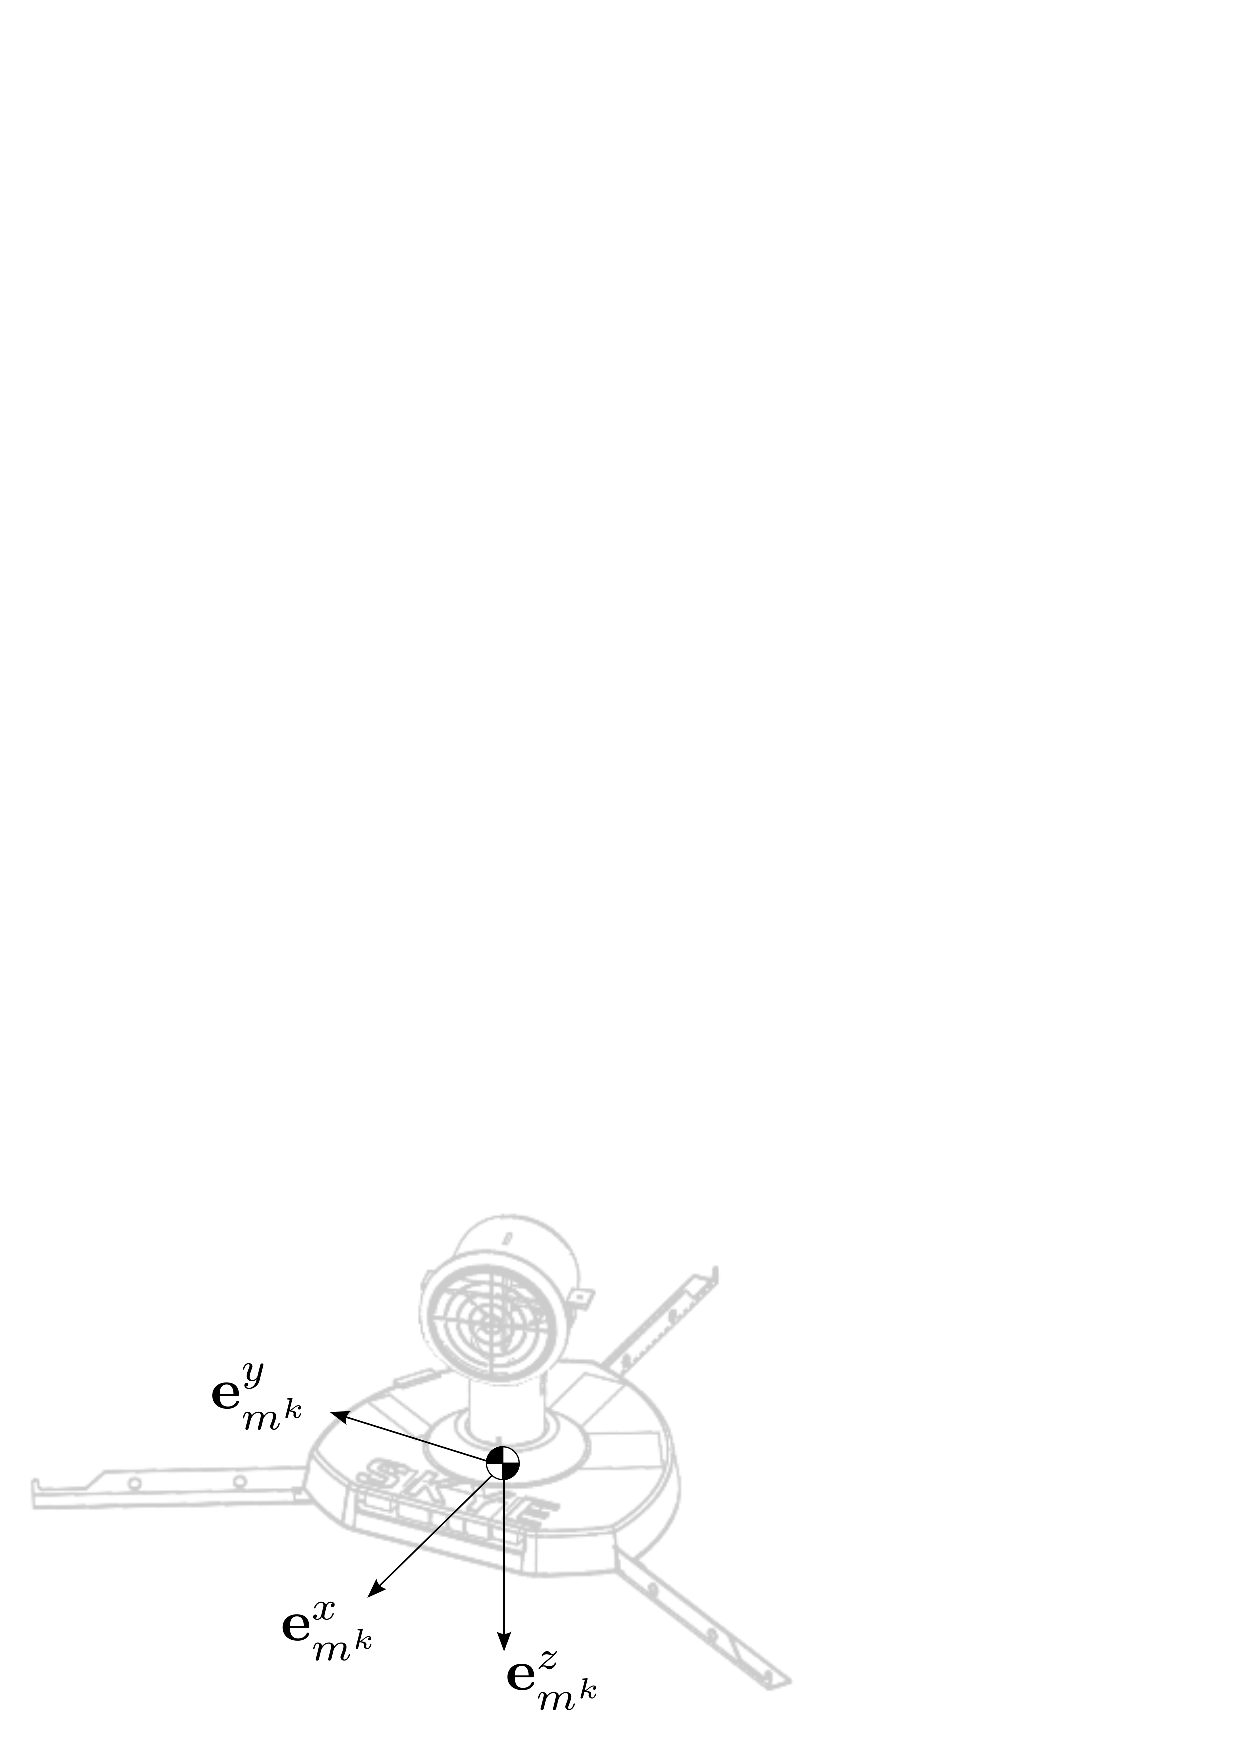
\includegraphics[width=.4\linewidth]{images/motor_frame.png}
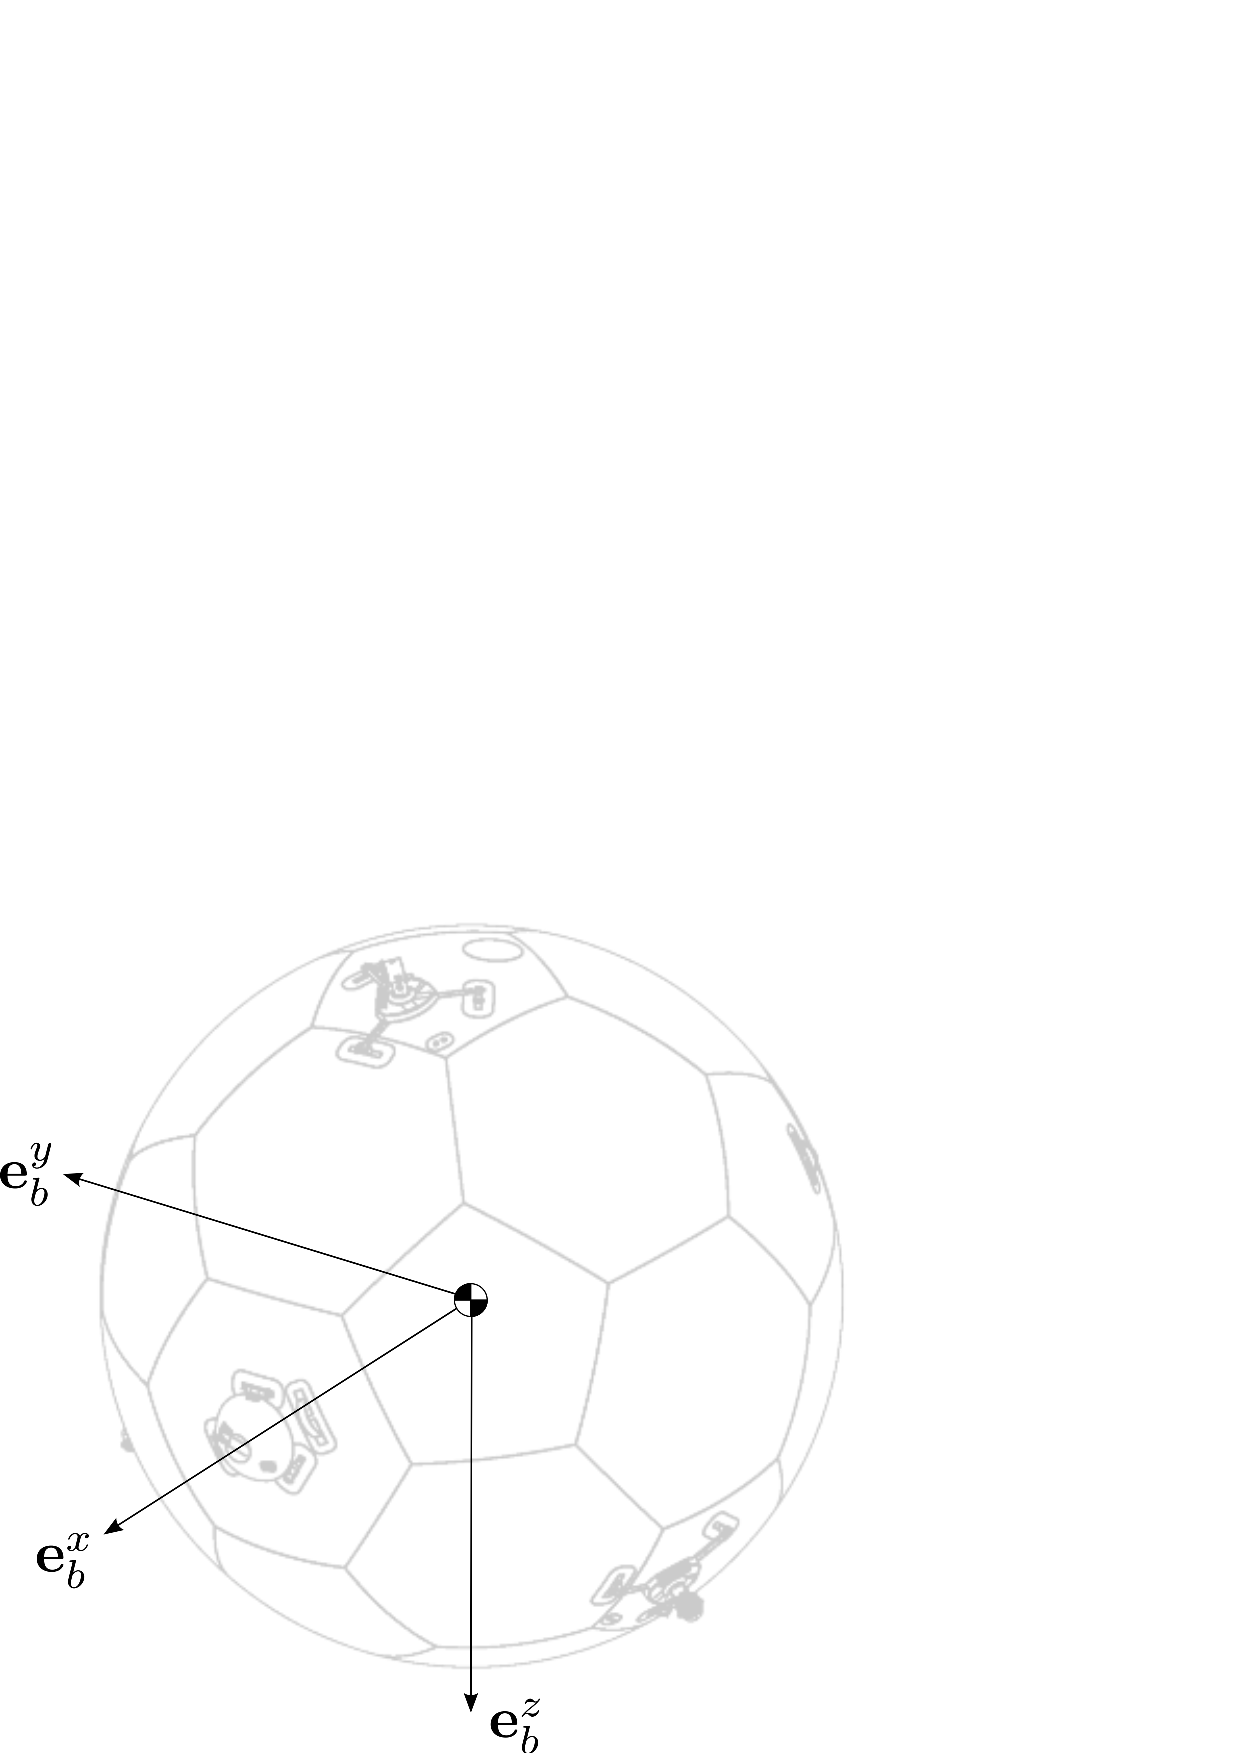
\includegraphics[width=.4\linewidth]{images/blimp_frame.png}
\caption{\textbf{Left}: Motor coordinate frame $b$. When the thruster is not rotated, it directs in $\mathbf{e}^x_{m_k}$ direction. $\mathbf{e}^z_{m_k}$ directs to the bottom. \textbf{Right}: Blimp coordinate frame $m_k$. $\mathbf{e}^x_{b}$ directs to the camera which is mounted at the front. $\mathbf{e}^x_{b}$ directs to the bottom.}
\end{figure}
